\documentclass[a4paper,12pt]{scrartcl}
\usepackage[utf8x]{inputenc}
\usepackage[T1]{fontenc} % avec T1 comme option  d'encodage c'est ben mieux, surtout pour taper du français.
%\usepackage{lmodern,textcomp} % fortement conseillé pour les pdf. On peut mettre autre chose : kpfonts, fourier,...
\usepackage[french]{babel, varioref} %Sans ça les guillemets, amarchpo
\usepackage{amsmath}
\usepackage{multicol}
\usepackage{amssymb}
\usepackage{tkz-tab}
\usepackage{exercice_sheet}
\flushbottom
\raggedbottom

%\trait
%\section*{}
%\exo{}
%\question{}
%\subquestion{}

\date{}

% Title Page
\title{Exercices sur les équations du 2\textsuperscript{nd} degré, corrigé}

\author{}

\begin{document}

\selectlanguage{french}

\maketitle

\exo{Résoudre les équations}

\question{}
$x^2 - 2x - 15$

$\Delta = b^2 - 4ac = (-2)^2 - 4 \times 1 \times (-15) = 64 > 0$

Donc l'équation a 2 solutions: 

$\sqrt{\Delta} = \sqrt{64} = 8$

$x_1 = \dfrac{2-8}{2} = -3$

$x_2 = \dfrac{2+8}{2} = 5$

On a donc: 

\Answer{$S = \left\lbrace -3 ; 5 \right\rbrace$}

\question{}
$4x(x+1) = -1$

Cette équation n'est pas de la forme $ax^2 + bx + c = 0$. Il faut donc la mettre en forme avant de pouvoir la résoudre.

$4x(x+1) = -1$

$\Leftrightarrow 4x^2 + 4x + 1 = 0$

Il s'agit là d'un cas particulier. On peut résoudre d'une autre façon: 

$4x^2 + 4x + 1$ est une identité remarquable $4x^2 + 4x + 1 = (2x+1)^2$.

L'équation est donc équivalente à: $(2x+1)^2 = 0$

Soit $2x+1 = 0$ (car si le carré d'un nombre est 0, alors ce nombre est 0)

$\Leftrightarrow x = -\dfrac{1}{2}$

\Answer{$S = \left\lbrace -\dfrac{1}{2} \right\rbrace$}

Bien-sûr, on peut résoudre cette équation en calculant $\Delta$ pou l'équation $4x^2 + 4x + 1 = 0$ trouvée après arrangement de l'équation de départ.


\question{}
$(2x-1)(x+1) = -6$

Telle quelle, on ne peut résoudre cette équation. Tout comme la précédente, il faut la développer puis mettre tous les éléments du même côté du signe $=$. 

$(2x-1)(x+1) = -6$

$\Leftrightarrow 2x^2 + 2x - x -1 +6 = 0$

$\Leftrightarrow 2x^2 + x +5 = 0$

$\Delta = b^2 - 4ac = 1^2 - 4 \times 2 \times 5 = -39 < 0$

Donc l'équation n'a pas de solution: 

\Answer{$S = \emptyset$}


\question{}
$2x^2 + x = 0$

Il s'agit également d'un cas particulier: $x$ est facteur commun. Ainsi, l'équation devient: 

$x(2x+1) = 0$ (équation produit)

\[ \Leftrightarrow
  \begin{cases}
   x      = 0 \\
   \text{ou} \\
   2x + 1 = 0 
  \end{cases}
\]

soit:

\[ \Leftrightarrow
  \begin{cases}
   x = 0 \\
   \text{ou} \\
   x = -\dfrac{1}{2} 
  \end{cases}
\]

\Answer{$S = \left\lbrace -\dfrac{1}{2} ; 0 \right\rbrace$}


\question{}
$(x+2)(x-1) = 0$

Il s'agit là d'une équation produit: 

\[ \Leftrightarrow
  \begin{cases}
   x+2 = 0 \\
   \text{ou} \\
   x-1 = 0
  \end{cases}
\]

\[ \Leftrightarrow
  \begin{cases}
    x = -2 \\
   \text{ou} \\
    x = 1 
  \end{cases}
\]

Donc:

\Answer{$S = \left\lbrace -2 ; 1 \right\rbrace$}

\exo{}

\question{}
Pour $x = 6$m, la largeur du rectangle $ABCD$ est 8m. L'aire du rectangle est donc $6 \times 8 = 48 \mbox{m}^2$.

\question{}
La hauteur du rectangle est $x$ et sa largeur $-2x + 20$. Son aire est donc $S(x) = x(-2x + 20) = -2x^2 + 20x$.

\question{}
\begin{table}[h]
\begin{center}
\begin{tabular}{|l|l|l|l|l|l|l|l|l|l|l|l|}
\hline
$x$    & 0 & 1  & 2  & 3  & 4  & 5  & 6  & 7  & 8  & 9  & 10 \\ \hline
$S(x)$ & 0 & 18 & 32 & 42 & 48 & 50 & 48 & 42 & 32 & 18 & 0  \\ \hline
\end{tabular}
\end{center}
\end{table}

\question{}
Représentation graphique de la fonction $S$, figure \vref{Cf}

\begin{figure}[h]
\begin{center}
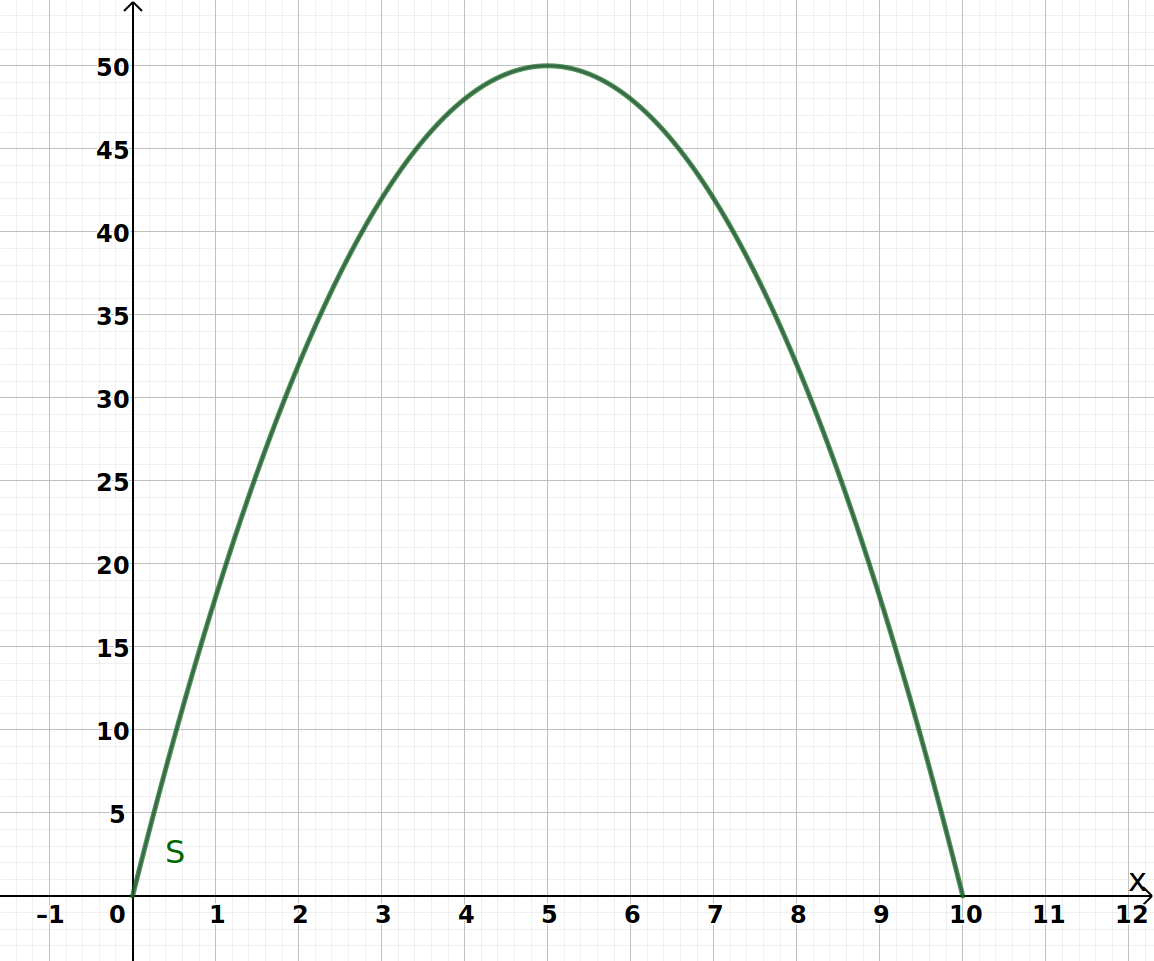
\includegraphics[width=0.6\textwidth]{pics/Cf.pdf}
\end{center}
\caption{Courbe $\mathcal{C}_S$, représentative de la fonction $S$}
\label{Cf}
\end{figure}

\question{}
Tableau de variation.

\subquestion{}
Pour commencer, on dérive la fonction $S$. 

$S'(x) = -4x + 20$

Ensuite, on cherche pour quelles valeurs de $x$ la dérivée est positive, ce qui revient à résoudre l'inéquation suivante: 

$S'(x) > 0$

$-4x + 20 > 0$

$\Leftrightarrow 20 > 4x$

$\Leftrightarrow 5 > x$

On peut donc en déduire le tableau de variation de la fonction $S$.

\begin{center}
\begin{tikzpicture}
   \tkzTabInit{$x$ / 1 , $S'(x)$ / 1 , $S(x)$ / 2}{$0$, $5$, $10$}
   \tkzTabLine{, +, z, -, }
   \tkzTabVar{-/ $0$, +/ $50$, -/ $0$}
\end{tikzpicture}
\end{center}


\subquestion{}
$S(x)$ atteint sa valeur maximale en $x = 5$, et ce maximum vaut $50$.

\question{}
Résolution graphique.

\subquestion{}

\begin{figure}
\begin{center}
\includegraphics[width=0.8\textwidth]{pics/Cf_equa.pdf}
\end{center}
\caption{Résolution graphique de l'équation $S(x) = 37.5$}
\label{Cf_equa}
\end{figure}

On voit figure \vref{Cf_equa} que $S(x)$ atteint la valeur $37.5$ pour $x=2.5$ et $x=7.5$. 

\subquestion{}
$-2x^2 + 20x = 37.5$

$\Leftrightarrow -2x^2 + 20x - 37.5 = 0$ %%%%%%%%%%%%

On reconnaît une équation polynomiale du second degré. 

$\Delta = 20^2-4 \times (-2) \times (-37.5)$

$\Delta = 100 > 0$ donc l'équation a 2 solutions.

$\sqrt{\Delta} = \sqrt{100} = 10$

$x_1 = \dfrac{-20 - 10}{-4} = 7.5$

$x_2 = \dfrac{-20 + 10}{-4} = 2.5$

On a donc : 

\Answer{$S = \left\lbrace 2.5 ; 7.5 \right\rbrace$}

%\exo{Résoudre les équations suivantes}
%
%\question{}
%$\Delta = 64 > 0$, donc le polynôme a donc 2 solutions.
%
%$\sqrt{\Delta} = 8$
%
%$x_1 = -3$
%
%$x_2 = 5$
%
%\Answer{$S = \left\lbrace -3 ; 5 \right\rbrace$}
%
%\question{}
%$\Delta = -39 < 0$, donc le polynôme n'a pas de solution.
%
%
%
%\question{}
%
%\question{}
%
%\question{}
%
%\question{}
%



\end{document}
